\begin{figure*}[t]
    \centering
    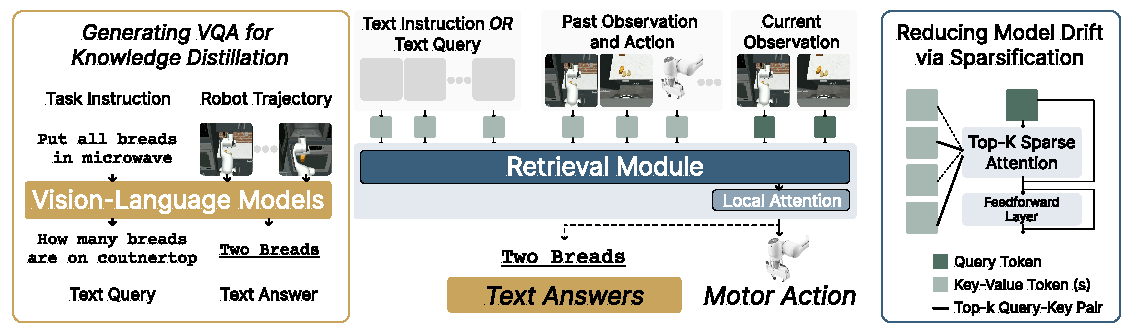
\includegraphics[width=\textwidth]{figures/method_overview_new.pdf}
    \vspace{-20pt}
    \caption{\textbf{Overview.} \ourmethod{} learns a visuomotor policy that retrieves information from the past observations and actions to predict low-level robot actions (middle), guided by priors from vision-language models to retrieve task-relevant information through VQA (left) and uses sparse attention to reduce model drift (right).}
    \label{fig:method_overview}
    \vspace{-10pt}
\end{figure*}